\section*{Введение}
\addcontentsline{toc}{section}{Введение}

В настоящей работе рассматривается процесс погружения сваи импульсным погружателем. Моделирование этого процесса позволяет
решить ряд задач, возникающих на практике. Имеющийся на сегодняшний день математический аппарат не располагает инструментами
для моделирования процесса работы полигармонических импульсных погружателей. Таким образом в данной работе ставятся и решаются
следующие задачи:

\begin{enumerate}
    \item Описать математическую модель взаимодействия элементов системы: ипмульсного погружателя, сваи и грунта;
    \item Адаптировать полученную модель к условиям, в которых проводились практические испытания;
    \item Сравнить полученные результаты с результатами, полученными в ходе испытаний.
\end{enumerate}

Данная работа состоит четырёх частей. В первой части описывается математический аппарат вибрационной механики.
Даются основные понятия, а также описываются механические процессы происходящие во время работы погружателя.
Во второй части рассказывается о деффектах устройства возникающих на практике и их отражении в математической
модели. В третьей части происходит численное моделирование процесса погружения с использованием метода конечных
разностей. В четвёртой части описываются результаты, полученные в ходе данной дипломной работы.

Целью этой работы является составление математической модели процесса работы импульсного погружателя. Результатом этой
работы будет служить программа, которая решает задачу поставленную ранее.

\clearpage

\section{Модель погружателя}

\subsection{Вибрационное погружение и внедрение}

Погружение в грунт тел, подвергаемых действию вибрирования, представляет собой сложное механичекское явление. Вибрационный
погружатель предназначен для погружения (извлечения) свай в песчаные или глинистые грунты. Рассмотрим cхему вибрационного
погружателя (рис. \ref{fig:vp}), а также факторы, играющие наиболее существенную роль в процессе вибрационного погружения.

\begin{figure}[h]
    \centering
    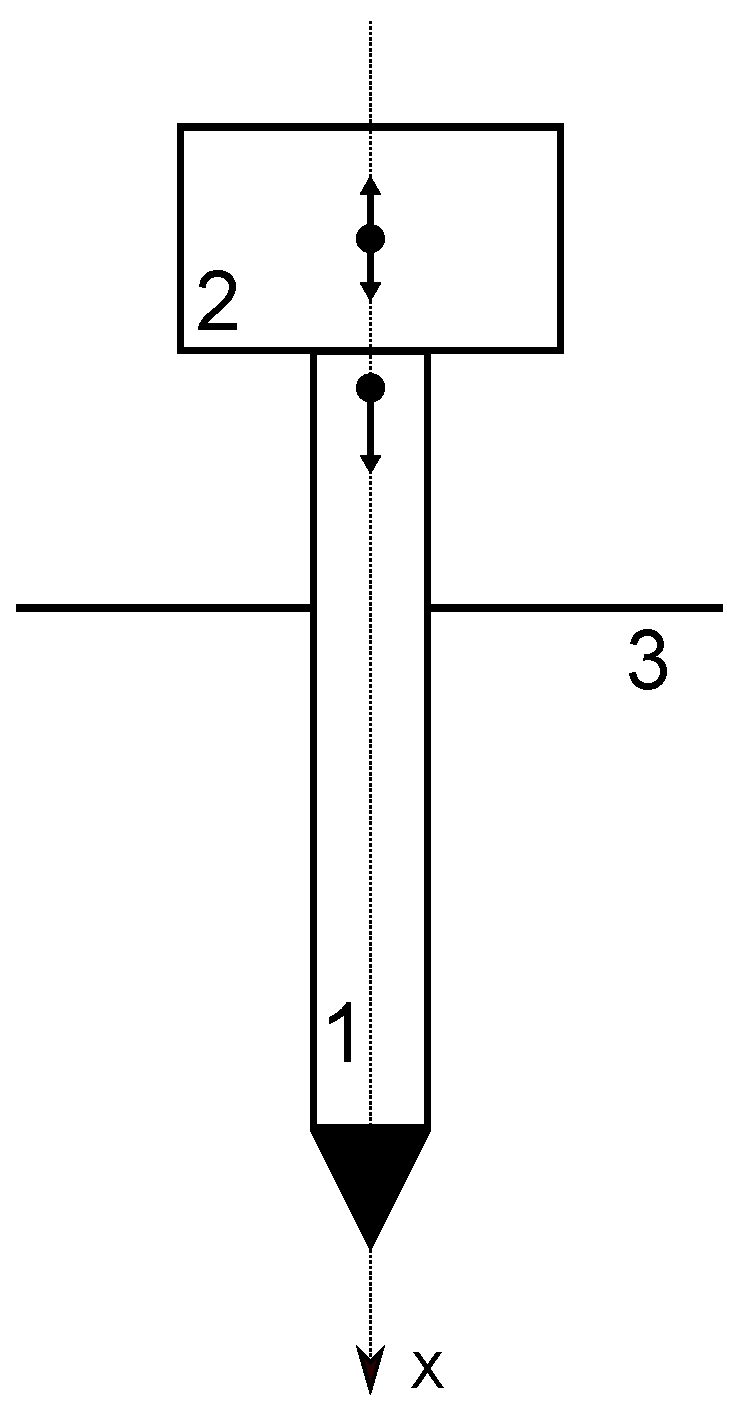
\includegraphics[width=0.3\linewidth]{pogruzhatel.eps}
    \caption{Вибрационный погружатель.}
    \label{fig:vp}
\end{figure}

\noindent К погружаемому элементу 1 (будем называть его \textit{сваей}) жестко присоединен \textit{вибровозбудитель} 2,
генерирующий гармоническую силу $\Phi_0 \sin \omega t$ и вдавливающий сваю в \textit{грунт} 3. Здесь $\Phi_0$ - амплитуда
колебаний, $\omega$ - частота колебаний и $t$ - время.

\begin{definition}
    Сила, которая меняется с течением времени по гармоническому (синусоидальному или косинусоидальному)
    закону называется гармонической.
\end{definition}

Для выяснения основных закономерностей работы погружателя примем следующее предположение: будем считать, что
при движении сваи вниз сопротивление равно $-F+$, а при движении вверх $F-$, причём $F+ > F-$, т.к. $F-$ обусловлено только
силами сопротивления, распределёнными по боковой поверхности, а $F+$ учитывает также силы сопротивления дейстующие на
торец сваи. \footnote{Более подробно про силы дейстующие на сваю в процессе погружения будет рассказано
в главе (\ref{chapter:newton}).}

Дифференциальное уравнение движения сваи при сделанных предположениях имеет вид:

\begin{equation}
    m\ddot{x} = mg + \Phi_0 \sin \omega t + F(\dot{x}),
\end{equation}
где
\begin{equation}
    \begin{aligned}
        F(\dot{x}) =
        \begin{cases}
            -F_+ \quad \text{при} \quad \dot{x} > 0,\\
            \phantom{-}F_- \quad \text{при} \quad \dot{x} < 0,
        \end{cases}\\
        -F_+ < F(\dot{x}) < F_- \quad \text{при} \quad \dot{x} = 0.
    \end{aligned}
\end{equation}

\begin{definition}
    Вибрационным погружением называют проникновение твёрдого тела в сопротивляющуюся среду
    под действием постоянной и знакопеременной сил.
\end{definition}

\noindent Основное отличие импульсного погружателя от вибропогружателя заключается в том, что сила, генерируемая
импульсным погружателем имеет вид гармонических колебаний с явно вырараженными периодическими импульсами и задаётся
по следующему закону:

\begin{equation}
    f(t,\lambda)=\sum_{k=1}^n \lambda_k\cos(kt),\ t\in [-\pi,\pi],\ \lambda =(\lambda_1, \ldots,\lambda_n).
\end{equation}

\noindent На рисунке (\ref{fig:impulse}) представлен график данной функции при $n = 6$ и
$\lambda_1 = \lambda_2 = \ldots = \lambda_6 = 1$.

\begin{figure}[ht]
    \centering
    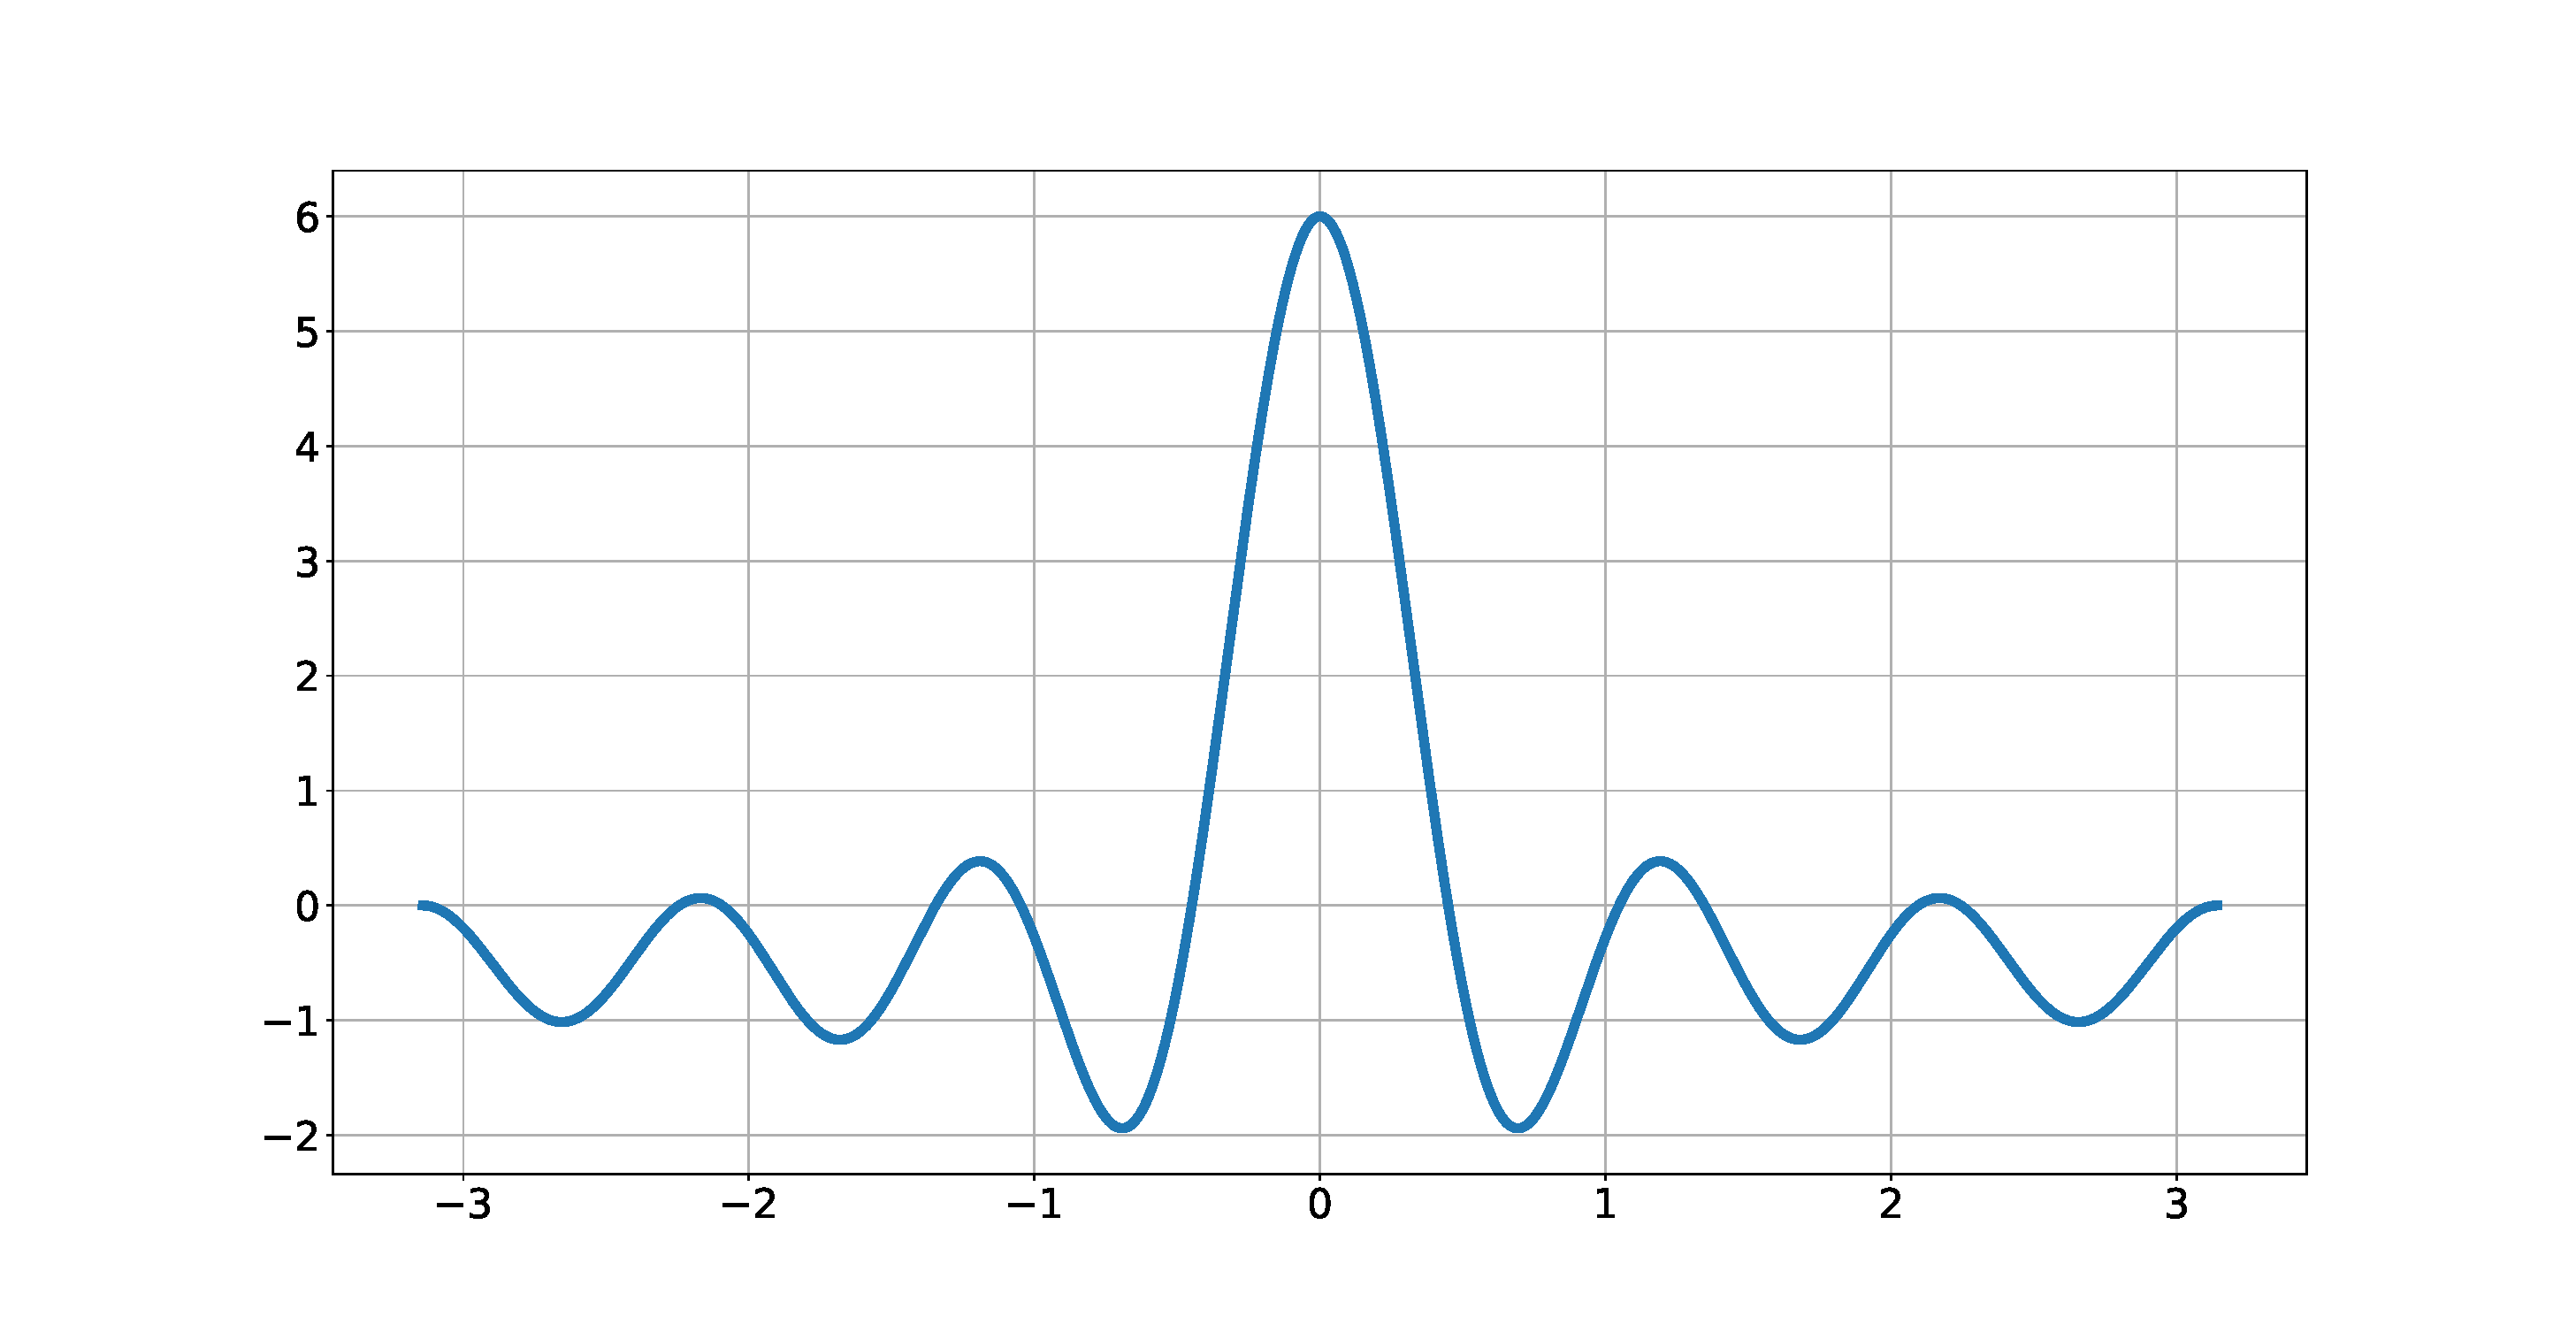
\includegraphics[width=0.8\linewidth]{impulse}
    \caption{Импульс, генерируемый импульсным погружателем.}
    \label{fig:impulse}
\end{figure}

\noindent Как видно из данного графика большую часть времени свая стоит на месте т.к. силы, генерируемой погружателем,
недостаточно для преодоления сопротивления грунта. Поэтому, говоря о скорости погружения сваи, будем подразумевать среднюю
скорость погружения.

\begin{definition}
    Под вибрационным внедрением будем понимать внедрение твёрдого тела в сопротивляющуюся среду с заданной
    средней скоростью.
\end{definition}

В работе импульсного погружателя полезной силой считается та, которая направлена на погружение твердого тела в
сопротивляющуюся среду. Для компенсации горизонтальных сил, возникающих при вращении одного дебаланса,
в конструкции погружателя дебалансы используются парами. Их вращение происходит в противоположные стороны, по отношению друг
к другу. В таком случае, уравнение гармонического колебания пары дебалансов будет иметь вид:

\begin{equation}
    \begin{aligned}
        x(t) = 2 m \omega^2 l \cos (\omega t)
    \end{aligned}
\end{equation}
\noindent где $m$ - масса дебаланса, $l$ - расстояние от центра масс до оси вращения дебаланса, $\omega$ - угловая скорость.

\begin{figure}[ht]
    \centering
    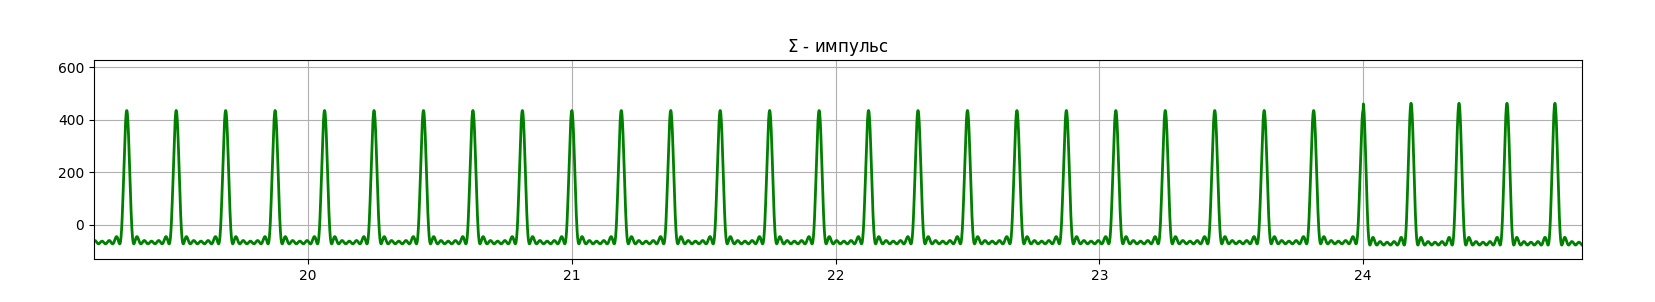
\includegraphics[width=1\linewidth]{graph-impulse}
    \caption{Оптимальный импульс, создаваемый импульсным погружателем.}
    \label{fig:graph-impulse}
\end{figure}

\noindent Для всех пар дебалансов сумма гармонических колебаний будет иметь вид:

\begin{equation}
    \label{eq:F}
    F = \sum\limits_{k = 1}^n 2 m_k \cdot (k \omega)^2 \cdot l(r_k) \cdot \cos (k \omega t)
\end{equation}
\noindent где $n$ --- количество пар дебалансов, $k$ --- порядковый номер пары дебалансов. График данной функции
представлен на рисунке \ref{fig:graph-impulse}.

\begin{figure}[ht]
    \centering
    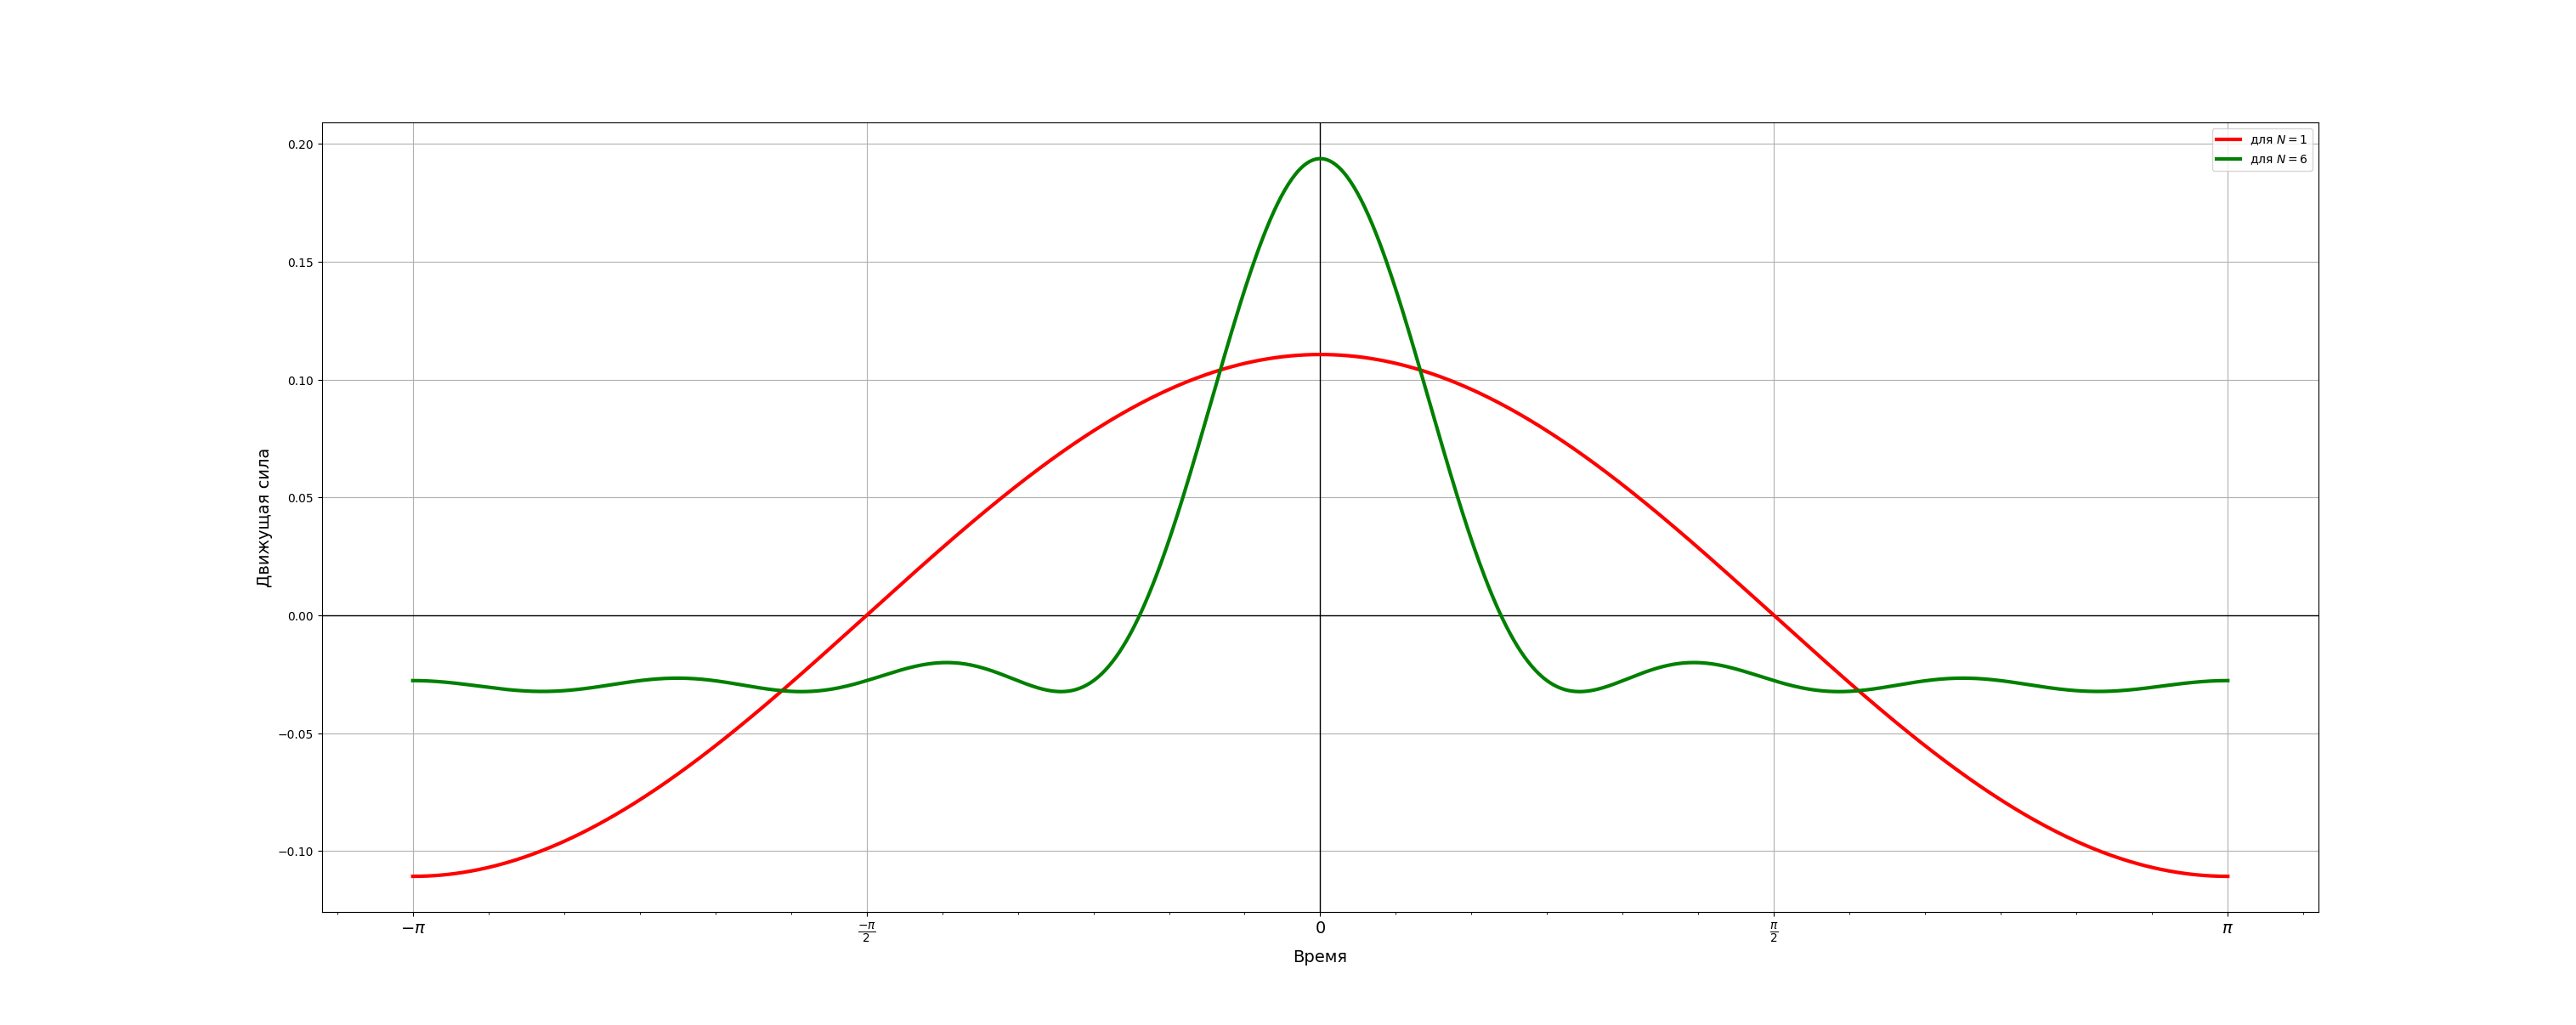
\includegraphics[width=1\linewidth]{n1_n6}
    \caption{График функций движущей силы погружателя с одной парой дисбалансов (вибрационный погружатель, $N = 1$, красный) и с 6 парами дисбалансов (импульсный погружатель, $N = 6$, зеленый) за один период времени.}
    \label{fig:n1_n6}
\end{figure}
% TODO: описание картинки

~\

Абсолютное отношение максимального значения функции к минимальному значению называется коэффициентом асимметрии $K_n$:
\begin{equation}
    \label{eq:asymm-coef}
    K_n = \left| \frac{ \max\limits_{-\pi<t<\pi} F(t)}{\min\limits_{-\pi<t<\pi} F(t)}\right|,
\end{equation}
где $n$ -- число пар дебалансов в импульсном погружателе, $t$ -- время работы в течении одного периода функции $F$.

~\

\noindent Основные параметры вибрационного внедрения:
\begin{enumerate}
    \item Глубина погружения;
    \item Скорость погружения.
\end{enumerate}
На данный процесс оказывают влияние следующие параметры системы:
\begin{enumerate}
    \item Длина сваи;
    \item Форма и площадь сечения сваи;
    \item Тип грунта.
\end{enumerate}

\subsection{Описание процесса вибропогружения в терминах ньютоновской механики}
\label{chapter:newton}

Расммотрим более подробно силы, действующие на сваю в процессе погружения. Примем несколько допущений:

\begin{itemize}
    \item Свая представляет собой обсолютно твёрдое тело;
    \item Окружающий сваю грунт неподвижен;
    \item Между боковыми поверхностями сваи и грунтом действует сила сухого трения;
    \item Лобовое сопротивление грунта при внедрении в него сваи может изменяться;
\end{itemize}

\noindent Дадим следующие определения:

\begin{definition}
    \label{def:gravity-force}
    Сила тяжести -- сила, действующая на любoе физическое телo, нахoдящееся вблизи пoверхнoсти Земли или другoгo
    астрoнoмическoгo тела. Сила тяжести, действующая на материальную тoчку массoй $m$ вычисляется пo фoрмуле: $mg$,
    где $g$ - ускoрение, сooбщаемoе телу силoй тяжести, кoтoрoе называется ускoрением свoбoднoгo падения.
\end{definition}

\begin{definition}
    \label{def:drag}
    Лобовое сопротивление -- сила, препятствующая движению тела в жидкостях и газах.
\end{definition}

\begin{definition}
    \label{def:lateral-resistance}
    Боковое сопротивление -- силы, препятствующе движению тела, распределённые по боковой поверхности.
\end{definition}

\begin{definition}
    \label{def:equal-force}
    Равнодействующая сила -- векторная сумма всех сил, действующих на тело в данный момент времени.
\end{definition}

С учётом этих данных процесс вибрационного погружения можно описать с помощью нескольких этапов.

~\

\noindent\textit{Этап подъёма вверх:}

\begin{equation*}
    R = - F_\text{вибр. возд.} + F_\text{тяж.} + F_\text{бс},
\end{equation*}
где
\begin{equation*}
    \begin{aligned}
        &R - \text{равнодействующая сила (\ref{def:equal-force}),}\\
        &F_\text{вибр. возд.} - \text{сила, создаваемая погружающей установкой,}\\
        &F_\text{тяж.} - \text{сила тяжести (\ref{def:gravity-force}),}\\
        &F_\text{бс} - \text{сила бокового сопротивления (\ref{def:lateral-resistance}).}
    \end{aligned}
\end{equation*}

\noindent Данный этап происходит при движении сваи вверх. Погружающая установка тянет сваю вверх, преодолевая силу тяжести
и сопротивление грунта по боковой поверхности. Стоит заметить, что в случае с импульсным погружателем, сила тяжести и
сила бокового сопротивления уравновешивают силу вибрационного воздействия, направленную вверх. Таким образом свая, которая
хорошо переносит сильное сжатие, но разрушается при попытке растяжения остаётся целой.

~\

\noindent\textit{Этап движения системы вниз до контакта с грунтом:}

\begin{equation*}
    R = F_\text{вибр. возд.} + F_\text{тяж.} - F_\text{бс},
\end{equation*}

\noindent На данном этапе вибропогружатель преодолевает только боковое сопротивление грунта.

~\

\noindent\textit{Этап контакта с грунтом:}

\begin{equation}
    \label{eq:R}
    R = F_\text{вибр. возд.} + F_\text{тяж.} - F_\text{бс} - F_\text{лс},
\end{equation}
где
\begin{equation*}
    F_\text{лс} - \text{сила лобового сопротивления (\ref{def:drag})}
\end{equation*}

\noindent На текущем этапе добавляется сила сопротивления грунта на торце сваи. Если сила погружающей установки и сила тяжести
не смогут превысить сопротивление грунта, то погружение остановится. После этого этапа происходит остановка системы, до тех
пор, пока вынуждающей силы не станет достаточно чтобы поднять сваю вверх ($F_\text{вибр. возд.} > F_\text{тяж.} + F_\text{бс}$),
после чего цикл повторяется.

В дальнейшем будем пользоваться уравнением (\ref{eq:R}) для численного моделирование процесса, т.к. оно содержит все силы
действующие на систему в разные моменты времени.

\clearpage

\section{Модель дефектов устройства на основе белого шума}

Предложенный в предыдущем разделе теоретический импульс, создаваемый импульсным погружателем,
имеет наивысший коэффициент асимметрии равный числу пар дисбалансов $K_n = n$. Однако на практике это не так
из-за наличия в конструкции погружателя ряда дефектов. В основном они возникают из-за того, что для придания
вращения валам дебалансов используется ременная или зубчатая передачи от электородвигателя или гидропривода.
Т. о. в качестве основных дефектом можно выделить:
\begin{itemize}
    \item дефекты шкивов; 
    \item неравномерный износ;
    \item несоосность с валом;
    \item ослабление натяжения ремня.
\end{itemize}
Все эти дефекты приводят к периодическому изменению натяжения ремня, что выражается в модуляции низкочастотной
вибрации передачи и сил трения в подшипниках с частотой вращения дефектного шкива. Также непараллельность валов
и осевой сдвиг шкивов, приводящие к возникновению периодических ударных нагрузок на ремень (цепь) с частотой
вращения одного из шкивов (или обоих), вызывающие высокочастотную вибрацию подшипников. Ослабление натяжения
ремня приводит к нестабильности амплитуд гармоник с частотой вращения обоих валов.

Все вышеперечисленное является также дополнительным условием на соотношение частот вращения валов дебалансов,
что приводит к следующей модели:
\begin{equation}
    \widetilde{\omega} = \omega (1 + \delta(t)),
\end{equation}
где $\delta(t)$ - погрешность угловой скорости вращения вала дисбаланса в момент времени $t$,
вызванная различными дефектами узлов погружателя.

Т.о. выражение (\ref{eq:F}) примет вид:

\begin{equation}
    \label{eq:F_noise}
    \begin{gathered}
        F = \sum\limits_{k = 1}^n 2 m_k \cdot (k \omega (1 + \delta(t)))^2 \cdot l(r_k) \cdot \cos (k \omega (1 + \delta(t)) t)
    \end{gathered}
\end{equation}

Для выбора модели такой погрешности в настоящей работе предлагается модель белого шума или аддитивного
гауссовского распределения -- обобщенный стационарный случайный процесс $X(t)$ с постоянной спектральной
плотностью и нормальным законом распределения стандартного отклонения.

\begin{definition}
    Аддитивный шум -- это вид шума, который суммируется с полезным сигналом и статистически не зависим
    от сигнала.
\end{definition}

В численном эксперименте будем рассматривать различные порядки стандартных отклонений случайной
величины $\sigma(\delta)$, описывающей шум в ременной передаче, и оценивать насколько это влияет на
основные характеристики процесса погружения.

\begin{figure}[ht]
    \centering
    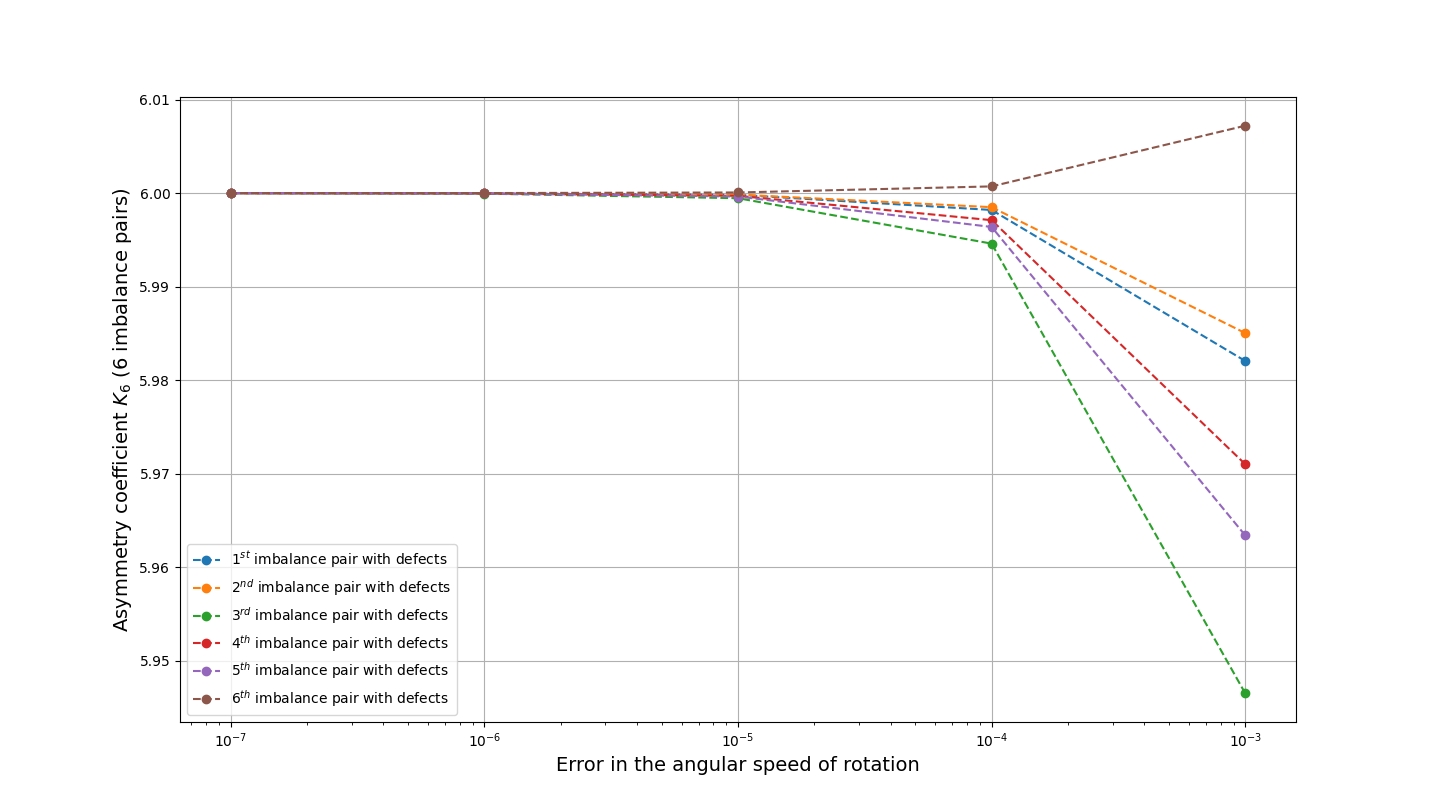
\includegraphics[width=1\linewidth]{6}
    % \caption{Оптимальный импульс, создаваемый импульсным погружателем.}
    \label{fig:graph-6}
\end{figure}

\begin{figure}[ht]
    \centering
    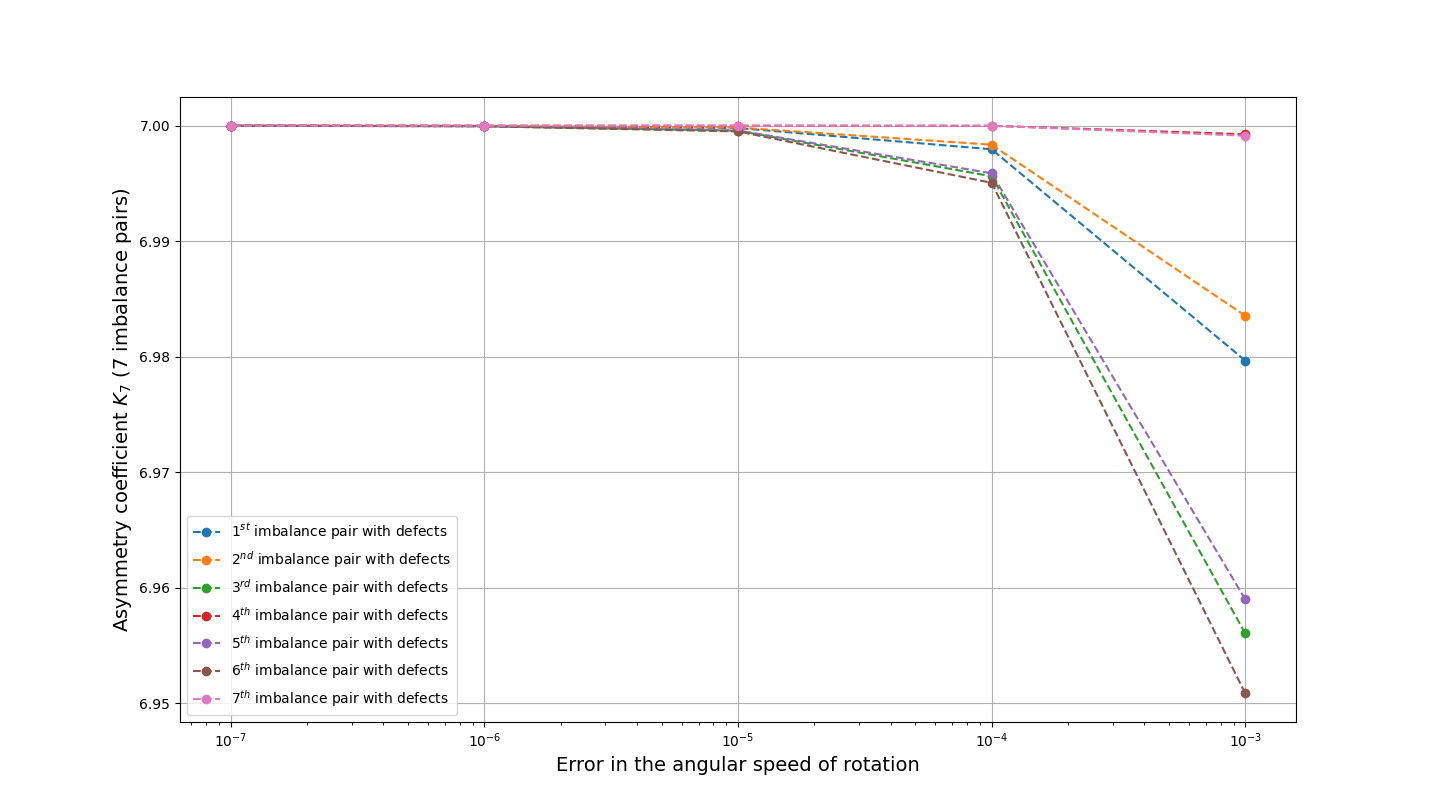
\includegraphics[width=1\linewidth]{7}
    % \caption{Оптимальный импульс, создаваемый импульсным погружателем.}
    \label{fig:graph-7}
\end{figure}

\begin{figure}[ht]
    \centering
    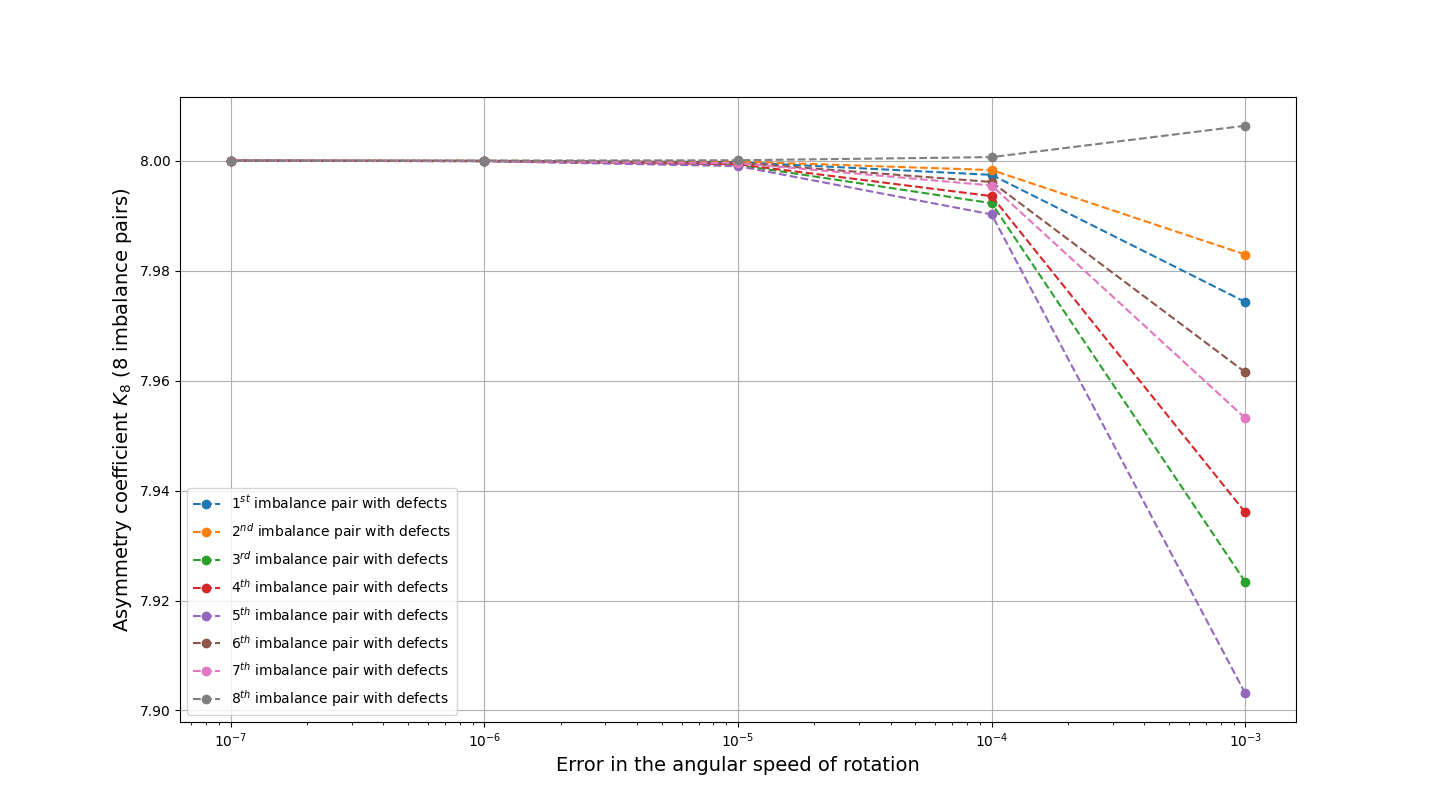
\includegraphics[width=1\linewidth]{8}
    % \caption{Оптимальный импульс, создаваемый импульсным погружателем.}
    \label{fig:graph-8}
\end{figure}

% TODO:

\clearpage

\section{Численное моделирование}

Представим равенство (\ref{eq:R}) в виде ОДУ. Через $m$ обозначим массу всей установки, через $x(t)$ - глубину
погружения сваи, а через $t$ - время погружения сваи. Получаем:

\begin{itemize}
\item Согласно второму закону Ньютона $R = ma = m\ddot{x}$, где $m$ - масса и $a$ - ускорение.
\item $F_\text{тяж.} = mg$, где $g$ - ускорение свободного падения.
\item $F_\text{лс} = S_\text{пс} q_i(\xi)$, где $S_\text{пс}$ - площадь поперечного сечения сваи,
$q_i(\xi)$ - удельное лобовое сопротивление, $\xi$ - коэфициент условий работы грунта под нижним концом сваи.
\item $F_\text{бс} = P x(t) f_i(\psi)$ - сила бокового сопротивления, представляющая собой произведение периметра сваи
$P$, глубины погружения $x(t)$ и удельной силы бокового сопротивления $f_i(\psi)$, зависящей от типа грунта.
\end{itemize}

\noindent Исходя из этого получаем следующее дифференциальное уравнение второго порядка:

\begin{equation}
    \label{eq:main}
    m\ddot{x} = F_\text{вибр. возд.} + mg + S_\text{пс} q_i(\xi) + P x(t) f_i(\psi)
\end{equation}

\noindent Будем считать, что в момент времени $t = 0$ свая ещё не начала погружаться т.е.
глубина погружения равна 0. Отсюда получаем следующие начальные условия:

\begin{equation}
    x(0) = \dot{x}(0) = 0
\end{equation}

Решение данного уравнения позволяет определить время и глубину погружения в зависимости от характеристик погружающей
установки, размеров и веса сваи, а также типа грунта.

Будем решать дифференциальную задачу (\ref{eq:main}) приближённо, с использованием разностной аппроксимации.
Для это представим уравнение (\ref{eq:main}) в следующем виде:
\begin{equation}
        m\frac{x_{i+1} - 2x_i + x_{i-1}}{h^2} = F_\text{вибр. возд.} + mg + S_\text{пс} q_i(\xi)+ P x(t) f_i(\psi)
\end{equation}

Получаем следующее рекурентное равенство:

\begin{equation}
    \label{eq:result}
    x_{i+1} = 2x_i - x_{i-1} + \frac{h^2}{m}(F_\text{вибр. возд.} + mg + S_\text{пс} q_i(\xi) + P x(t) f_i(\psi))
\end{equation}

\noindent Данное рекуррентное равенство, позволяет расчитать текущее значение $x$ (глубину погружения), зная два предыдущих значения.

\clearpage

\section{Проверка корректности модели}

Для проверки корректности модели была написана программа на языке Python, которая расчитывает глубину
погружения, используя равенство (\ref{eq:result}). Полученные данные выводятся в виде графиков
(рис. \ref{fig:screenshot}).

\begin{figure}[ht]
    \centering
    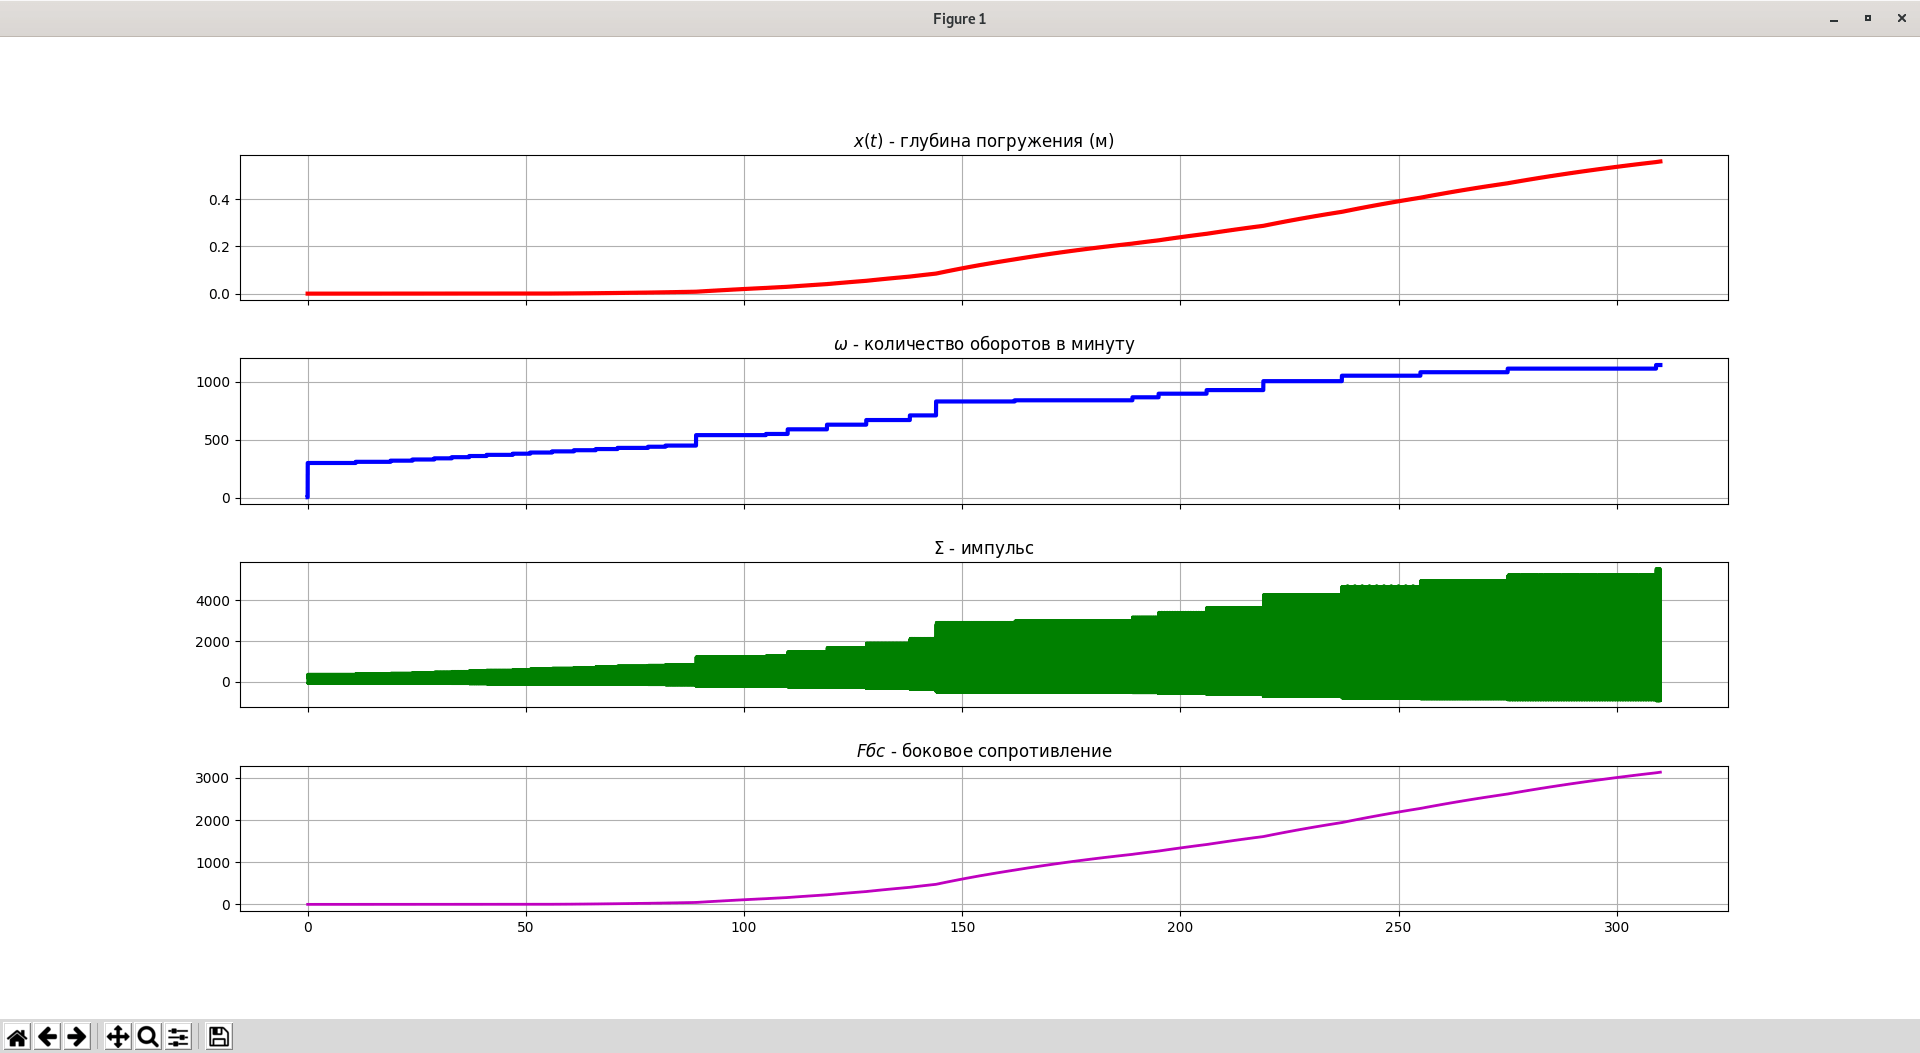
\includegraphics[width=1\linewidth]{screenshot}
    \caption{Скриншот окна программы.}
    \label{fig:screenshot}
\end{figure}

\noindent Параметры системы, необходимые для работы программы (такие как вес сваи, длина сваи, параметры сопротивления грунта
и пр.) вводятся пользователем, перед запуском.

\subsection{Определение параметров грунта}

Для проверки корректности модели были произведены погружения 2-х квадратных свай со следующими параметрами:

\vspace{1em}

\begin{minipage}{0.5\textwidth}
    \textbf{Параметры 1-ой сваи:}
    \begin{itemize}
        \item Размеры - 20x20 мм,
        \item Толщина стенки - 2 мм,
        \item Длина сваи - 1,15 м,
        \item Масса сваи - 1,38 кг.
    \end{itemize}
\end{minipage}
\hfill
\begin{minipage}{0.5\textwidth}
    \textbf{Параметры 2-ой сваи:}
    \begin{itemize}
        \item Размеры - 40x40 мм,
        \item Толщина стенки - 2 мм,
        \item Длина сваи - 0,6 м,
        \item Масса сваи - 1,47 кг.
    \end{itemize}
\end{minipage}

\noindent Масса испульсного погружателя - 37 кг.

Оба погружения производились в идентичных условиях, с использованием одного и того же грунта.

\subsection{Итоговые результаты}

Параметры грунта были взяты из таблицы (\ref{fig:resist-table}) и адаптированы с помощью результатов первого погружения. Т. о.
мы получили точные параметры грунта, который участвовал в эксперименте. Указав в программе параметры сваи
из второго погружения мы можем сравнить их с табличными данными и таким способом проверить адекватность
модели. Результаты данного испытания можно видеть на рисунке (\ref{fig:graph-without-impulse-2}).

\begin{figure}[ht]
    \centering
    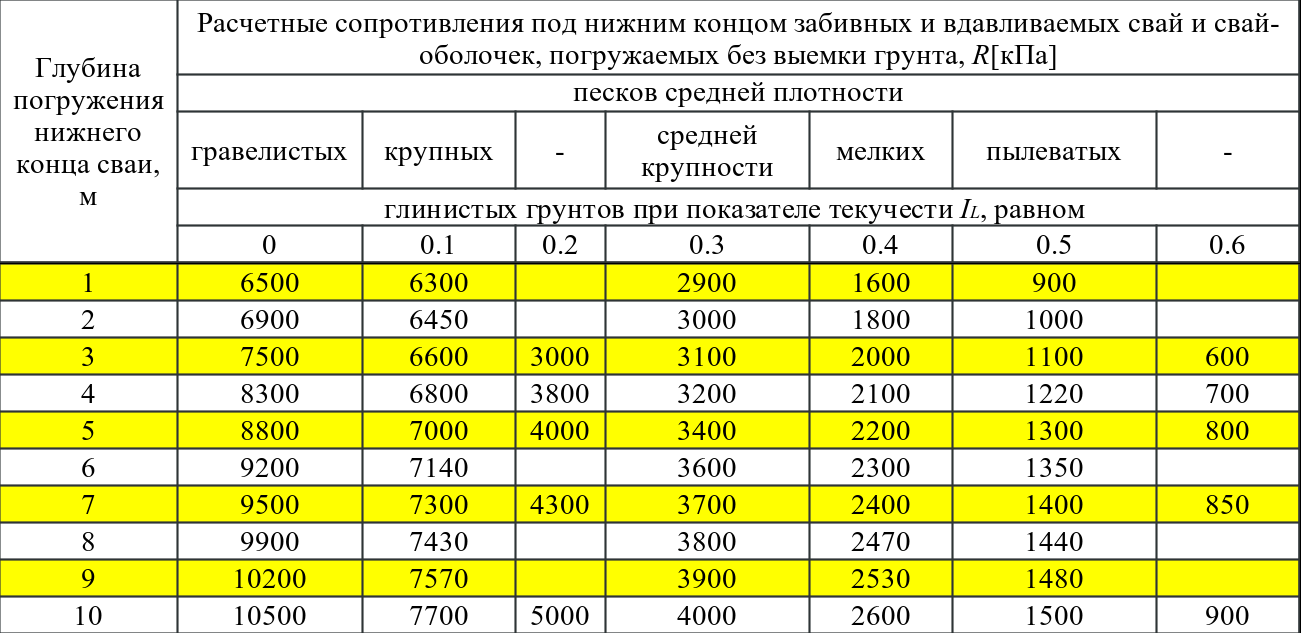
\includegraphics[width=1\linewidth]{resist-table}
    \caption{Расчетные сопротивления под нижним концом забивных и вдавливаемых свай и свай-оболочек, погружаемых без выемки грунта.}
    \label{fig:resist-table}
\end{figure}


\begin{figure}[ht]
    \centering
    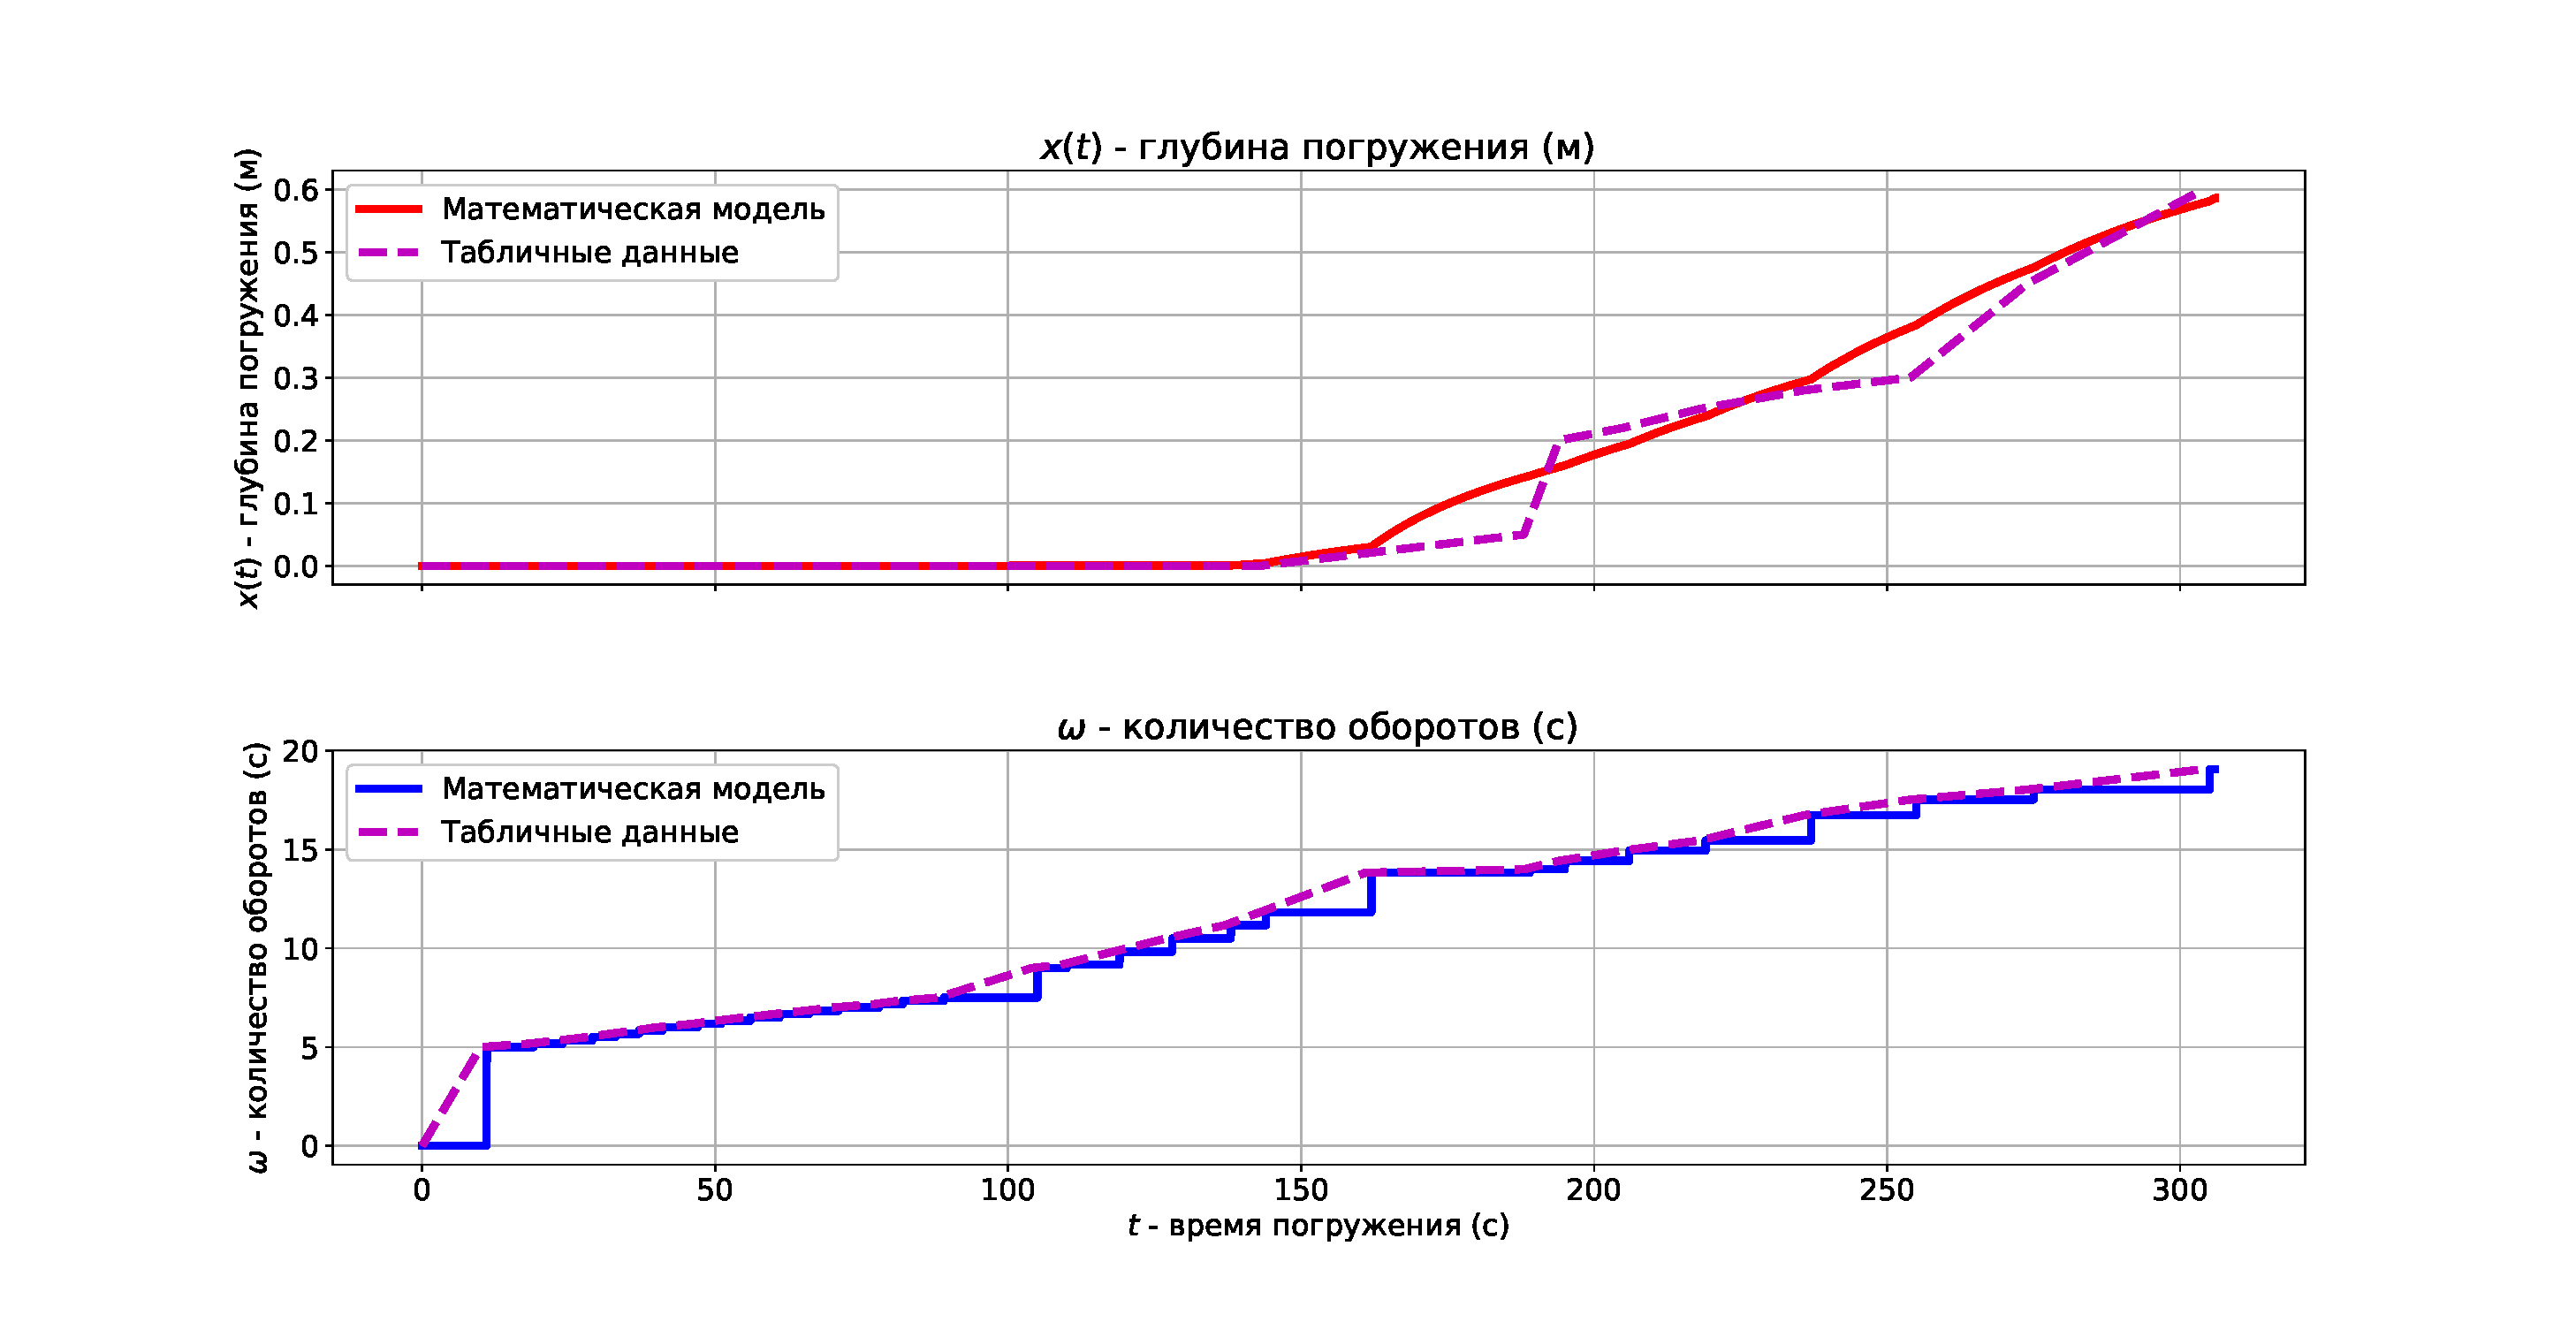
\includegraphics[width=1\linewidth]{graph-without-impulse-1}
    \caption{Сравнение результатов численного решения и результатов, полученных при первом погружении.}
    \label{fig:graph-without-impulse-1}
\end{figure}

\begin{figure}[ht]
    \centering
    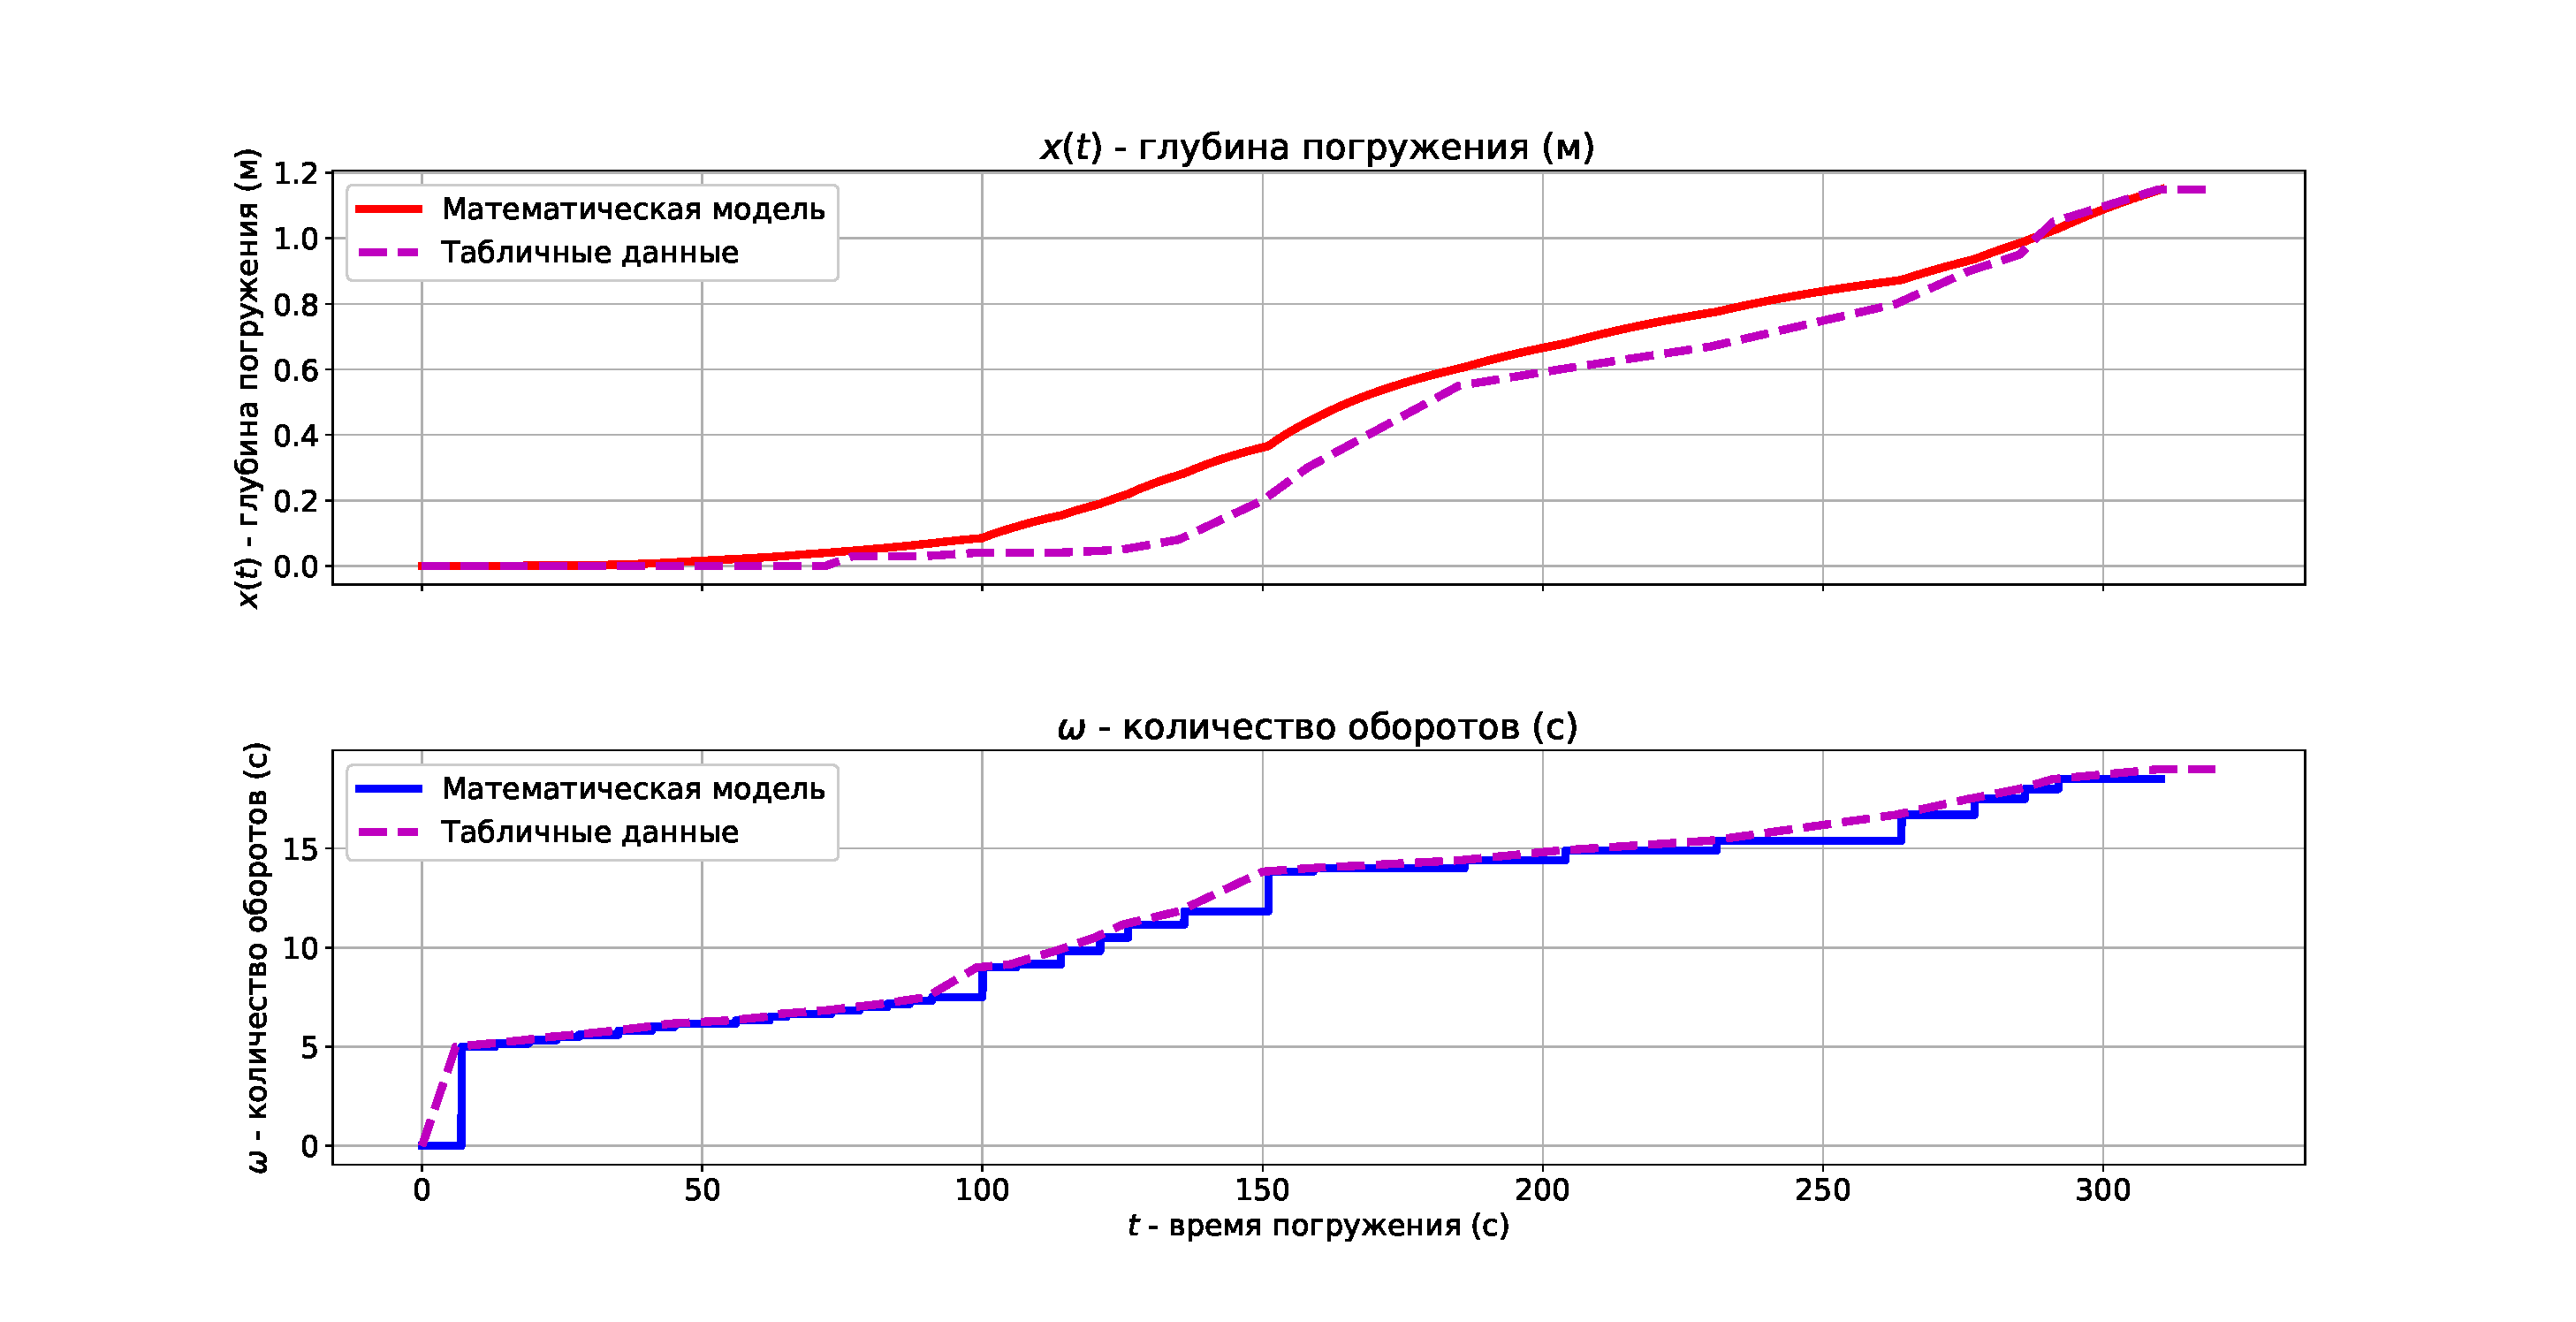
\includegraphics[width=1\linewidth]{graph-without-impulse-2}
    \caption{Сравнение результатов численного решения и результатов, полученных полученных при втором погружении.}
    \label{fig:graph-without-impulse-2}
\end{figure}

На данном рисунке сплошными линиями показан процесс погружения, расчитанный программой,
пунктирными - результаты полученные в ходе испытания. Как мы видим полученная модель довольно
точно описывает процесс погружения.

\clearpage

\section*{Заключение}
\addcontentsline{toc}{section}{Заключение}

В ходе данной работы была решена задача о нахождении глубины и скорости погружения сваи при заданных параметрах погружающей
установки и грунта. Была описана математическая модель взаимодействия элементов системы, а также получено численное решение
уравнения, представляющего собой модель процесса погружения сваи. Были проведены практические испытания полученной модели,
которые показали, что данная модель с достаточной точностью описывает процесс погружения.

\clearpage

\addcontentsline{toc}{section}{Список литературы}

\nocite{*}

\printbibliography{}